145. \begin{figure}[ht!]
\center{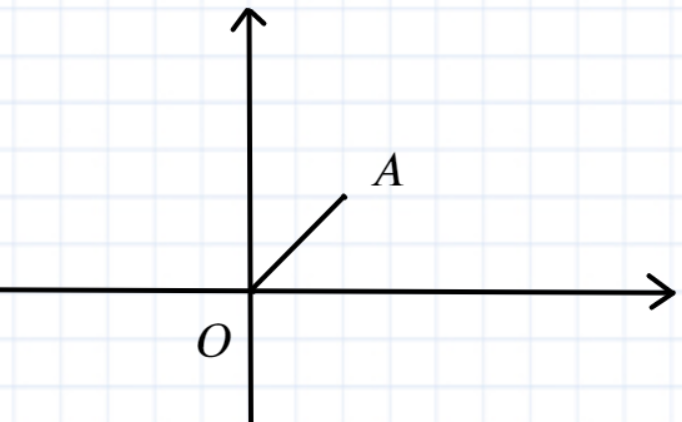
\includegraphics[scale=0.35]{g8-144.png}}
\end{figure}\\
Высота, опущенная из точки $O$ на $AB,$ равна 2. Тогда $S_{\Delta OAB}=\cfrac{1}{2}\cdot 2 \cdot AB=4,\ AB=4.$ Тогда абсцисса точки $B$ может быть равна либо $2+4=6,$ либо $2-4=-2,$ то есть у точки $B$ могут быть координаты $(6;2)$ или $(-2;2).$\\
